\documentclass{article}

% Language setting
% Replace `english' with e.g. `spanish' to change the document language
\usepackage[english]{babel}

% Set page size and margins
% Replace `letterpaper' with `a4paper' for UK/EU standard size
\usepackage[letterpaper,top=2cm,bottom=2cm,left=3cm,right=3cm,marginparwidth=1.75cm]{geometry}

% Useful packages
\usepackage{amsmath}
\usepackage{graphicx}
\usepackage[colorlinks=true, allcolors=blue]{hyperref}
\usepackage{float}

\usepackage{caption}
\usepackage{subcaption}


\begin{document}
\begin{titlepage}
   \begin{center}
       \vspace*{1cm}
        
        \Huge
        \textbf{DSE315/615: Data Science in Practice}

        \vspace{0.5cm}
        \huge
        Breast Cancer Prediction using Machine Learning
            
       \vspace{5cm}
        
        \Large
        \textbf{Akshat Singh}
        
        \textbf{20031}
        
        \vspace{0.5cm}
        
        \textbf{Varun Nair}
        
        \textbf{20303}
        
        \vspace{0.3cm}
        
        \textbf{\today}


        \vspace*{\fill}

        \begin{figure}[h]
            \centering
            
\includegraphics[width = 3cm]{Base/IISERB Logo.png}       
        \end{figure}
        
        \Large
       Indian Institute of Science Education and Research (IISER) Bhopal.\\
        India\\
       
            
   \end{center}
\end{titlepage}

\section{Introduction}

\footnote{Codes available at: \href{https://github.com/Borun2002/Breast-Cancer-Classification}{https://github.com/Borun2002/Breast-Cancer-Classification}}

Machine learning is a powerful tool that enhances efficiency by enabling computers to learn from data and make predictions or decisions without explicit programming. Its practical applications range from streamlining business processes and automating tasks to improving personalized recommendations in areas like entertainment and e-commerce. In healthcare, it aids in diagnostics and treatment planning by extracting valuable insights from complex medical data, showcasing its broad utility in optimizing various facets of our daily lives.

Breast cancer poses a significant global health challenge, necessitating innovative approaches for early detection and improved prognostic assessments. This project tries to use machine learning to predict the nature of breast cancer—whether benign or malignant.

\section{Objectives}

The primary goals of this project include developing a machine learning model that accurately classifies breast cancer cases as benign or malignant and assessing the model's performance against established metrics.

\section{Data Collection}

Data for this project were sourced from the UCI ML repository, a widely recognized platform for Machine Learning Data, accessible through the following link: \href{http://archive.ics.uci.edu/dataset/17/breast+cancer+wisconsin+diagnostic}{UCI ML repository}. This repository is renowned for hosting diverse datasets, providing a valuable resource for machine learning practitioners and researchers.

\section{Preprocessing}

The provided data exhibited no missing values; therefore, no processing was required. Principal component analysis was conducted, and the top 15 components were selected based on the analysis of the scree plot shown in fig \ref{fig:scree} Subsequently, features were standardized for each model.

\begin{figure}[H]
    \centering
    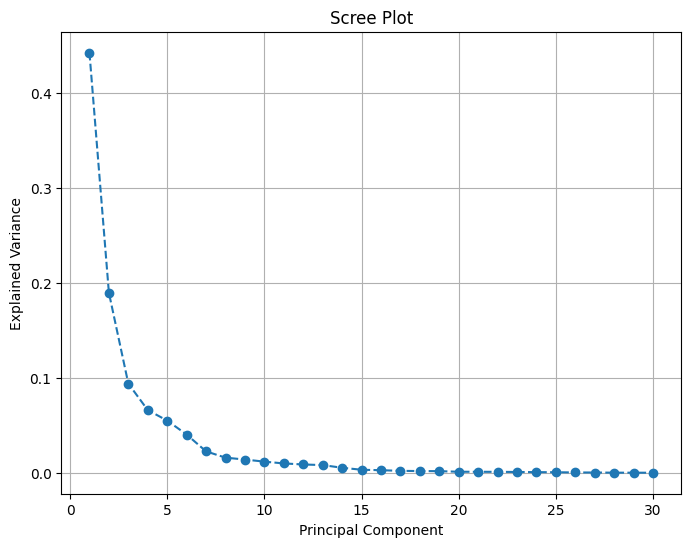
\includegraphics[width = 0.6\linewidth]{Images/scree.png}
    \caption{Scree Plot for PCA analysis}
    \label{fig:scree}
\end{figure}

\section{Exploratory Data Analysis}

The dataset has 30 features, including things like radius and texture, each with three values. We noticed strong connections, especially between radius, perimeter, and area. The three radius values (radius1, radius2, and radius3) were pretty similar, so we're thinking about making things simpler by either removing similar features or using something called Principal Component Analysis (PCA).

On the analysis of each feature in people with benign and malignant tumors. It was observed that people with malignant tumors generally had higher average values for feaures with same names(radius1, radius2, and radius3) as shown in fig \ref{fig:mean-radius} compared to those with benign tumors. This suggests these features might be important in telling apart benign and malignant tumors.

\begin{figure}[H]
    \centering
    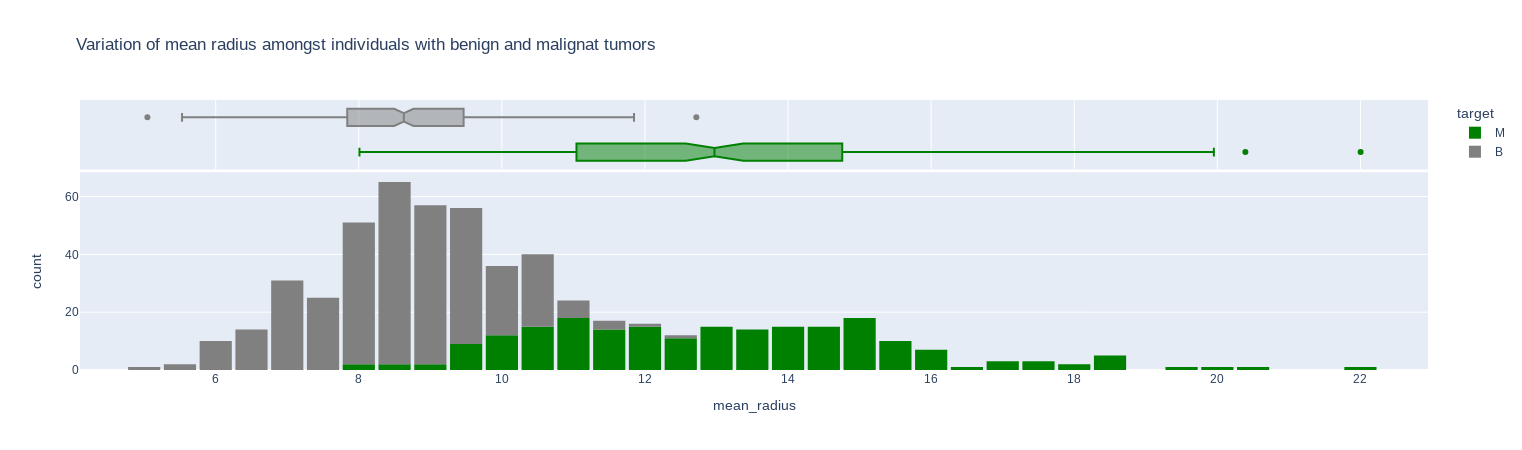
\includegraphics[width = 0.9\linewidth]{Images/mean_radius.png}
    \caption{Variation of mean radius}
    \label{fig:mean-radius}
\end{figure}

\section{Model Selection}

The following classification models were used for training and on each of these models, hyper-parameter tuning was done and the parameters with the best accuracy scores were chosen.:

\begin{itemize}
    \item \textbf{Baseline Classifier:} The baseline classifier used here is a majority class classifier which predicts the most frequent class in the training data for every instance. No hyper-parameter tuning was used as it is the reference model.
    
    \item \textbf{Decision Tree Classifier:} A decision tree classifier is a model that recursively splits the dataset based on features, making decisions at each node to classify instances into different classes.

    \item \textbf{Support Vector Machine Classifier:} A Support Vector Machine (SVM) classifier is a model that aims to find a hyperplane that best separates classes in the feature space, making it effective for both linear and non-linear classification tasks.

    \item \textbf{K-Nearest Neighbours Classifier:} A K-Nearest Neighbors (KNN) classifier is a model that classifies instances based on the majority class of their k-nearest neighbors in the feature space.

    \item \textbf{Logistic Regression Classifier:} A Logistic Regression classifier is a linear model that uses the logistic function to model the probability of belonging to a particular class, making it suitable for binary and multi-class classification tasks.

    \item \textbf{Random Forest Classifier:} A Random Forest Classifier is an ensemble model that consists of a collection of decision trees, where each tree is trained on a random subset of the data. It combines their predictions to improve overall performance and robustness.

    \item \textbf{Bagging Classifier:} A Bagging Classifier is an ensemble model that combines multiple base classifiers, typically decision trees, trained on random subsets of the training data. It averages or takes a majority vote of the predictions to improve overall model performance and reduce overfitting. Here decision tree was used.

    \item  \textbf{Voting Classifier:} A Voting Classifier is an ensemble model that combines the predictions of multiple individual classifiers, often of different types, using a majority vote (hard voting) or weighted average (soft voting) to make the final prediction. Here, Decision tree, SVM, KNN, Logistic Regression, Random Forest and Bagging Classifiers were used for both hard and soft voting.

    \item \textbf{Stacking Classifier:} A Stacking Classifier is an ensemble model that combines multiple base classifiers by training a meta-classifier to make predictions based on the outputs of the individual classifiers. It involves stacking the predictions of the base classifiers as additional features for training the meta-classifier. Here, Decision tree, SVM, KNN, Logistic Regression, Random Forest and Bagging Classifiers were used for the training.
    
\end{itemize}

Other than these classification models, 4 clustering models were used to check how good they are compared to the classification models if no labels are there, for all the models the number of clusters were set to 2. The models were:

\begin{itemize}
    \item \textbf{K-Means}: K-Means is an unsupervised machine learning algorithm used for clustering. It partitions the input data into k clusters by iteratively assigning each data point to the cluster whose centroid is closest and updating the centroids based on the mean of the points in each cluster.

    \item \textbf{Agglomerative Clustering:} Agglomerative Clustering is an unsupervised machine learning algorithm used for hierarchical clustering. It starts with each data point as a singleton cluster and iteratively merges the closest pairs of clusters until only one cluster remains. The linkage criterion (e.g., ward, complete, average) determines how the distance between clusters is calculated during merging.
    
    \item \textbf{BIRCH:} BIRCH (Balanced Iterative Reducing and Clustering using Hierarchies) is an unsupervised machine learning algorithm for hierarchical clustering. It is designed for large datasets and incrementally builds a tree structure to represent the clusters. BIRCH is memory-efficient and suitable for streaming data, making it well-suited for scenarios with high-dimensional datasets.

    \item  \textbf{Spectral Clustering:} Spectral Clustering is an unsupervised machine learning algorithm used for clustering. It works by transforming the data into a spectral domain, where clusters are identified based on the eigenvalues of the similarity matrix. Spectral clustering can be particularly effective for datasets with complex structures or non-convex shapes.

\end{itemize}

\section{Results}

After hyper-parameter tuning, the final accuracy and f1-score of the models are as follows(for clustering, the clusters are compared with labels):

\begin{table}[H]
    \centering
    \begin{tabular}{|c|c|c|}
        \hline
        \textbf{Model} & \textbf{Accuracy} & \textbf{f1-score}\\
        \hline
        Baseline Classifier & 0.64 & 0.79 \\
        \hline
        Decision Tree Classifier & 0.96 & 0.94 \\
        \hline
        SVM Classifier & 0.94 & 0.91 \\
        \hline
        KNN Classifier & 0.88 & 0.80 \\
        \hline
        Logistic Regression & 0.94 & 0.91 \\
        \hline
        Random Forest Classifier & 0.92 & 0.89 \\
        \hline
        Bagging Classifier & 0.95 & 0.93 \\
        \hline
        Voting Classifier(Hard) & 0.94 & 0.91 \\
        \hline
        Voting Classifier(Soft) & 0.93 & 0.90 \\
        \hline
        Stacking Classifier & 0.94 & 0.91 \\
        \hline
        K-Means Cluster & 0.90 & 0.92 \\
        \hline
        Agglomerative cluster & 0.63 & 0.01 \\
        \hline
        BIRCH Cluster & 0.84 & 0.88 \\
        \hline
        Spectral Cluster & 0.63 & 0.01 \\
        \hline
    \end{tabular}
    \caption{Different Models and their accuracy and f1-score}
    \label{tab:result}
\end{table}

\begin{figure}[H]
    \begin{subfigure}[b]{0.45\textwidth}
        \centering
        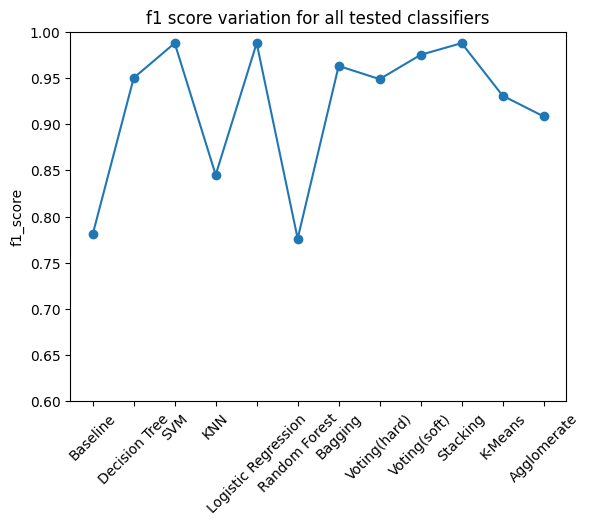
\includegraphics[width = \textwidth]{Images/f1.png}
        \caption{f1 scores of all models}
        \label{fig:f1}
     \end{subfigure}
     \begin{subfigure}[b]{0.45\textwidth}
        \centering
        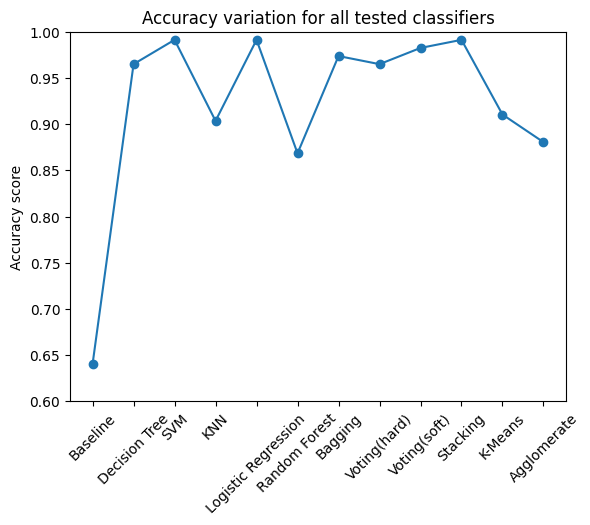
\includegraphics[width = \textwidth]{Images/acc.png}
        \caption{Accuracy of all models}
        \label{fig:accuracy}
     \end{subfigure}

\end{figure}

\section{Conclusion}


After a thorough analysis and comparison of various models, it has been determined that \textbf{Decision Tree} Model had the best accuracy and f1-score among the models used. Hence this is selected as the final model.

This is a practical selection as the data is not balanced and Decision Trees excel with imbalanced datasets, they adeptly model non-linear boundaries without being influenced by class distribution. Their flexibility in handling diverse data patterns, insensitivity to skewed class proportions, interpretability, and natural treatment of missing values make them a fitting choice.

Additionally, noteworthy insights emerged regarding the performance of clustering algorithms. Although not surpassing the efficacy of classification algorithms, clustering demonstrated decent results. Despite limited exploration in this area, it is acknowledged that clustering algorithms could serve as viable options in scenarios where labeled training data is scarce or unavailable.

\end{document}